\documentclass{article}
\usepackage{amsmath} 
\usepackage{graphicx} 
\usepackage{authblk}
\usepackage{url}
\usepackage{hyperref}
\usepackage{multirow}
\usepackage{amssymb}
\usepackage{subcaption}
\usepackage[linesnumbered,boxed]{algorithm2e}

\topmargin 0.0cm
\oddsidemargin 0.2cm
\textwidth 16cm 
\textheight 21cm
\footskip 1.0cm

\title{Numerical Method for Ordinary Differential Equations with Initial Conditions and Its Application in Physics}
\author[1]{Mengzhi Chen}
\author[1]{Tong Li}
\affil[1]{Department of Physics and Astronomy, Michigan State University}
\date{}

\begin{document}
	\maketitle
	\begin{abstract}\label{abstract}
	Ising model is a simple but important model to explain ferromagnetism. 
However, only one- and two-dimensional cases have been solved analytically. 
Therefore, it is necessary to develop a numerical method for the simulation of Ising model. 
In this work we focus on the application of Metropolis algorithm to the solve two-dimensional (2D) Ising model. 
We benchmark our numerical results with the analytical solution, 
and confirm that the system has a proper probability distribution and converges quickly to equilibrium in our simulation. 
The behaviors of phase transition around critical temperature also agree well with the analytical solution, 
and the critical temperature of infinitely large lattice is estimated to be 2.265 from our simulation, 
which is quite close to the theoretical value 2.269. 
Our work shows the success of Metropolis algorithm in the simulation of Ising model and 
we can simply extend it to higher dimensions.  

	\end{abstract}

\section{Introduction}\label{intro} 
Ising model is a simple but important model for the explanation of magnetization. 
It assumes that atomic spins are located on a $N$-dimensional lattice grid, 
and these spins only have two discrete states, up ($\sigma=1$) or down ($\sigma=-1$). 
Only neighboring spins can interact with each other, and thus its Hamiltonian can be written as 
\begin{equation}\label{eq:hamiltonian}
H=-J\sum_{<kl>}^{N}\sigma_k\sigma_l\,,
\end{equation}
where $J>0$ and $<kl>$ indicates that we only sum over nearest neighbors. 
\par
In statistical physics, the equilibrium of a system described by Eq. \ref{eq:hamiltonian} should be solved using canonical ensemble, 
which involves a summation over all possible microscopic states to obtain the partition function. 
For $N$-dimensional Ising model with size $L$ in each dimension, 
the total number of all microscopic states is $2^{L^N}$, which cannot be simply summed over. 
The one- and two-dimensional cases has been solved analytically and they show several interesting properties of phase transition. 
But the exact solution of higher-dimensional Ising model is still unavailable, 
and thus numerical methods which avoid the summation over all possible states are required for the simulation of Ising model. 
\par
In this report, we discuss the Monte Carlo method for the simulation of two-dimensional (2D) Ising model 
and compare our results with the analytical solution. 
In Sec. \ref{theory} several properties shown in the analytical solution are discussed, for the comparison in Sec. \ref{results}. 
Sec. \ref{method} gives the outline of Monte Carlo algorithm we utilize for 2D Ising model, 
and then Sec. \ref{results} discusses the results of our simulation. 
Conclusions are given in Sec. \ref{conclude}. 

	
\section{Examples of ordinary differential problems in physics}\label{physcis_problem}
	
	\subsection{The Earth-Sun system}\label{earthsun}
	The Earth-Sun system is a two-body system governs by the attractive gravitational force between them
\begin{equation}
	\vec{F}_G = \frac{GM_{\mathrm{S}}M_{\mathrm{E}}\hat{r}}{r^2},
\end{equation}
where G is the gravitational constant; 
$M_{\mathrm{S}}$ and $M_{\mathrm{E}}$ are mass of the Sun and the Earth; $\vec{r}$ is the displacement between them.

Given the fact the Sun is about $10^6$ heavier than the Earth, we can safely keep the Sun as the center of mass (C.M.) in this problem. 
With a proper coordinate setup, the orbit of the Earth is co-planer in $xy$-plane. 
Using Newton's second law we get the following first-order ordinary differential equations (ODEs) for the Earth

\begin{equation}
	\label{earthsunodes}
	\left\{  
             \begin{array}{lr}  
             	\frac{dx}{dt} = v_x \\
				\frac{dx}{dt} = v_x \\
            	\frac{dv_x}{dt} = -\frac{GM_{\mathrm{S}}x}{r^3} \\
				\frac{dv_y}{dt} = -\frac{GM_{\mathrm{S}}y}{r^3}.
			\end{array}  
	\right.	
\end{equation}

By solving above equations, we can obtain the informations about the Earth's orbit we need.

	
	\subsection{Many-body problem}\label{quantumdot}
	In the above Sec. \ref{earthsun}, we simplify the calculation of the orbit of the Earth by taking into account only it's interaction with the Sun. 
This simplification is reasonable as the Sun is much heavier than other planets in the solar system. 

However, if we want to go a step further to get a more precise description of the Earth's orbit. 
We have to include distortions from other seven planets as well as the Pluto.
We should also abandon our previous static Sun approximation but using the real center of mass of the solar system.
Until now, we have a new set of ODEs for the Earth

\begin{equation}
	\left\{  
             \begin{array}{lr}  
             	\frac{dx}{dt} = v_x \\
				\frac{dy}{dt} = v_y \\
            	\frac{dv_x}{dt} = \sum\limits_{i=1}^{n}-\frac{GM_{\mathrm{i}}x_i}{r_i^3} \\
				\frac{dv_y}{dt} = \sum\limits_{i=1}^{n}-\frac{GM_{\mathrm{i}}y_i}{r_i^3},
			\end{array}  
	\right. 	
\end{equation}
where $i$ runs over all other celestial bodies except the Earth itself. 
Besides the Earth, we have similar sets of ODEs for every celestial body.

By solving these coupled ODEs, we can obtain a full description for the solar system.

	
\section{Numerical methods}\label{method}
  
	\subsection{Euler's forward method}\label{euler}
	Suppose a first-order ordinary differential equation

\begin{equation}
	\frac{dx}{dt} = f(x,t);\ t\in[t_0,t_1]
\end{equation}
with a initial value $x_0$ at time $t_0$. 

In order to solve this problem, we first discretize the region $ [t_0,t_1]$ into N subintervals with a step $h$, so we get the relation

\begin{equation}
	h=\frac{t-t_0}{N}.
\end{equation}
Then, We have discretized $x_i=x(t_i=t_0+ih)$ where $i$ is a integer between 0 and $N$.

Using Taylor expansion, we get 

\begin{equation}
	\label{eulerexpan}
	x_{i+1} = x_i + \frac{dx_i}{dt}h + \frac{d^2x_i}{dt^2}h^2 + O(h^3),
\end{equation}
where i goes from 0 to $N-1$.
The Euler's forward method truncates at the second term of the above equation.
Thus, Eq. \ref{eulerexpan} becomes

\begin{equation}
	\begin{aligned}
		x_{i+1} & = x_i + \frac{dx_i}{dt}h + O(h^2) \\ 
				& = x_i + f(x_i,t_i)h + O(h^2).
	\end{aligned}
\end{equation}
We can see it's a one-step method with a local error $O(h^2)$.

Getting back to the Earth-Sun system, we can formulate Eq. \ref{earthsunodes} to

\begin{equation}
	\left\{  
             \begin{array}{lr}  
             	x_{i+1} = x_i + v_x^{i}h \\
				y_{i+1} = y_i + v_y^{i}h \\
             	v_x^{i+1} = v_x^{i} - \frac{4\pi^2x_i}{r_i^3}h\\
             	v_y^{i+1} = v_y^{i} - \frac{4\pi^2y_i}{r_i^3}h.
			\end{array}  
	\right.	
\end{equation} 
in unit of AU for length, year (yr) for time and $M_{\mathrm{S}}$ for mass. 
We will keep using this unit system in our report and calculations. 
Starting from some initial conditions, we can simply solve out time evolution of the Earth iteratively. 
Our implementation of this method with a  circular orbit initial conditions is shown in Algorithm \ref{alg::euler}. 

\begin{algorithm}[tb]
	\caption{The Euler's forward method for the Earth-Sun system. It initials from a circular orbit.}
	\label{alg::euler}
	\KwIn{$x_0=1$, $y_0=0$, $v_{x}^0=0$, $v_{y}^0=2\pi$, $M_{\mathrm{E}}$, $M_{\mathrm{S}}$, $G$ }
	\KwOut{$\vec{x}$=($x_0$,$x_1$,...,$x_N$), $\vec{y}$, $\vec{v}_x$, $\vec{v}_y$, $\vec{E}_k$, $\vec{E}_p$, $\vec{E}$, $\vec{L}_z$} 
	$r$ = sqrt($x_0^2$+$y_0^2$)\;
	// $i$ is deferent time points $t_i=t_0+ih$\;
    \For{$i=1;i<=N;i++$}
    { $x_{i} = x_{i-1} + v_x^{{i-1}}h$;
    $y_{i} = y_{i-1} + v_y^{{i-1}}h$\;
    $v_x^{i} = v_x^{i-1} - \frac{4\pi^2x_{i-1}}{r_{i-1}^3}h$;
    $v_y^{i} = v_y^{i-1} - \frac{4\pi^2y_{i-1}}{r_{i-1}^3}h$\;
    $r$ = sqrt($x_i^2$+$y_i^2$)\;
    // Kinetic energy $E_k$, Potential energy $E_k$, Total energy $E$, Angular momentum in $\hat{z}$ $L_z$\;
    $E_k^i$ = 0.5$M_{\mathrm{E}}$($(v_x^{i})^2$+$(v_y^{i})^2$);
    $E_p^i$ = $-\frac{GM_{\mathrm{E}}M_{\mathrm{S}}}{r}$\;
    $E^i$ = $E_p^i$ + $E_k^i$;
    $L_z^i$ = $M_{\mathrm{E}}(x_iv_y^{i}-y_iv_x^{i})$\;
    }
	return $\vec{x}$, $\vec{y}$, $\vec{v}_x$, $\vec{v}_y$, $\vec{E}_k$, $\vec{E}_p$, $\vec{E}$, $\vec{L}_z$\;
\end{algorithm}

We can see that the Euler's forward method is easy to be realized.
 However, it has vital defects that it violates the energy conservation and time reversibility.
 The total energy increases with time in the Euler's forward method.
 That's why we need the Velocity-Verlet method to describe physical systems.

	
	\subsection{Velocity-Verlet method} \label{verlet}
	The velocity-Verlet method is widely used in molecular dynamics calculation as it overcomes these defects. It conserves energy with small round-off errors\cite{toxvaerd2012energy}.

Staring from the Taylor expansions under same discretization

\begin{equation}
	\begin{aligned}
		x_{i+1} = x_i + x_i^{(1)}h + x_i^{(2)}h^2 + O(h^3),\\
		v_x^{i+1} = v_x^{i} + v_x^{i(1)}h + v_x^{i(2)}h^2 + O(h^3),
	\end{aligned}
\end{equation}
with a initial value $x_0$ and $v_x^0$ at time $t_0$. We truncate at the third term and evaluate $v_x^{i(2)}h \approx v_x^{i+1(1)}-v_x^{i(1)}$. We can see that velocity-Verlet method is a two-step method with a local error $O(h^3)$

In the Earth-Sun system, with this method, we can formulate Eq. \ref{earthsunodes} to

\begin{equation}
	\left\{  
             \begin{array}{lr}  
             	x_{i+1} = x_i + v_x^{i}h - \frac{4\pi^2x_i}{r_i^3}\frac{h^2}{2} \\
				y_{i+1} = y_i + v_y^{i}h - \frac{4\pi^2y_i}{r_i^3}\frac{h^2}{2} \\
             	v_x^{i+1} = v_x^{i} - (\frac{4\pi^2x_i}{r_i^3}+\frac{4\pi^2x_{i+1}}{r_{i+1}^3})\frac{h}{2}\\
             	v_y^{i+1} = v_y^{i} - (\frac{4\pi^2y_i}{r_i^3}+\frac{4\pi^2y_{i+1}}{r_{i+1}^3})\frac{h}{2}.
			\end{array}  
	\right.	
\end{equation} 
We show our realization of the velocity-Verlet method in Algorithm \ref{alg::verlet}. Compared with the Euler forward method, we can see the calculations in this method is more complicated.

\begin{algorithm}[tb]
	\label{alg::verlet}
	\caption{The Velocity-Verlet method for the Earth-Sun system. It initials from a circular orbit.}
	\KwIn{$x_0=1$, $y_0=0$, $v_{x}^0=0$, $v_{y}^0=2\pi$, $M_{\mathrm{E}}$, $M_{\mathrm{S}}$, $G$ }
	\KwOut{$\vec{x}$=($x_0$,$x_1$,...,$x_N$), $\vec{y}$, $\vec{v}_x$, $\vec{v}_y$, $\vec{E}_k$, $\vec{E}_p$, $\vec{E}$, $\vec{L}_z$} 
	$r$ = sqrt($x_0^2$+$y_0^2$)\;
	$a_x^0$ = $\frac{4\pi^2x_{i-1}}{r_{i-1}^3}$;
    $a_y^0$ = $\frac{4\pi^2y_{i-1}}{r_{i-1}^3}$\;
	// $i$ is deferent time points $t_i=t_0+ih$\;
    \For{$i=1;i<=N;i++$}
    {$x_{i} = x_{i-1} + v_x^{i-1}h - \frac{a_x^0h^2}{2}$;
    $y_{i} = y_{i-1} + v_y^{i-1}h - \frac{a_y^0h^2}{2}$\;
    $r$ = sqrt($x_i^2$+$y_i^2$)\;
    $a_x^1$ = $\frac{4\pi^2x_{i}}{r_{i}^3}$;
    $a_y^1$ = $\frac{4\pi^2y_{i}}{r_{i}^3}$\;
    $v_x^{i} = v_x^{i-1} - \frac{(a_x^0+a_x^1)h}{2}h$;
    $v_y^{i} = v_y^{i-1} - \frac{(a_y^0+a_y^1)h}{2}h$\;
	$a_x^0$ = $a_x^1$;
    $a_y^0$ = $a_x^1$\;
    // Kinetic energy $E_k$, Potential energy $E_k$, Total energy $E$, Angular momentum in $\hat{z}$ $L_z$\;
    $E_k^i$ = 0.5$M_{\mathrm{E}}$($(v_x^{i})^2$+$(v_y^{i})^2$)\;
    $E_p^i$ = $-\frac{GM_{\mathrm{E}}}{r}$;
    $E^i$ = $E_p^i$ + $E_k^i$\;
    $L_z^i$ = $M_{\mathrm{E}}(x_iv_y^{i}-y_iv_x^{i})$\;
    }
	return $\vec{x}$, $\vec{y}$, $\vec{v}_x$, $\vec{v}_y$, $\vec{E}_k$, $\vec{E}_p$, $\vec{E}$, $\vec{L}_z$\;
\end{algorithm}

	
	\subsection{Object-oriented code development}\label{obj}
	For flexibility and extensivity of our codes, the idea of object-oriented programming is employed in the development. 
A class called "planet" stores all the properties of a planet, such as coordinate, velocity, acceleration, total force on it, 
angular momentum and energy. 
This class also contains functions to initialize before each time step, to calculate gravitational force between two objects, 
to add up these forces, to do one-step Euler's forward or Velocity-Verlet calculation and to update all the properties after each step. 
The user can fix one or more objects at a given position, 
or he/she can also call a friend function to move the center of mass to origin. 
All the parameters needed for planets in the solar system are given from command line and input file. 
	
\section{Results and discussion}\label{results}

	\subsection{Comparison between two methods}
	To test the stability of Euler forward (Euler) and the velocity-Verlet (VV) method, we initialize the Earth-Sun system with a circular orbit as stated in Algorithms \ref{alg::euler,alg::verlet}.

We varies the step size $h$ starting from 0.02 yr to 0.001 yr.
The Earth's orbits calculated by these two methods for 10 years are show in Fig. \ref{fig::earth}. 
Globally speaking, we see orbits given by the Euler method expand in time.  
On the other hand, VV methods' orbits keep circular with some tiny fluctuation hardly seen in Fig. \ref{fig:earth500}.
It justifies the our statements in Sec. \ref{method} that the VV method conserves energy but the Euler method increase energy.

For a large step size in Fig. \ref{fig:earth500}, the Euler method is very unstable. Its orbit deviates from circle both in distance and shape apparently. 
As the step size becomes smaller, we can see that the Euler method becomes better; as the orbits expand slower and slower from \ref{fig:earth500} to Fig. \ref{fig:earth10000}.
 The trends we observed agree with the statement that the error in the Euler method goes down with decreasing $h$. We can hardly see differences between orbits yielded from the VV method, which indicates the it's stability.
 
\begin{figure}[tb]
	\begin{subfigure}[tb]{0.5\textwidth}
		\centering
		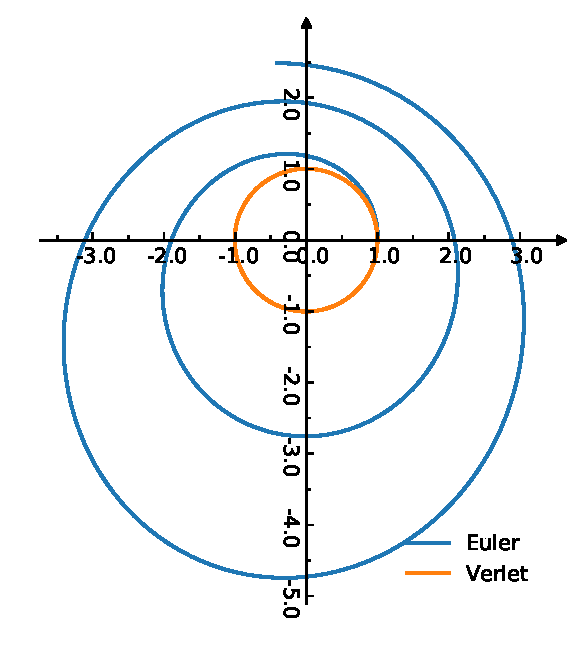
\includegraphics[width=0.7\textwidth]{Earth500.eps}
		\caption{$h = 0.02$yr}
		\label{fig:earth500}
	\end{subfigure}
~
	\begin{subfigure}[tb]{0.5\textwidth}
		\centering
		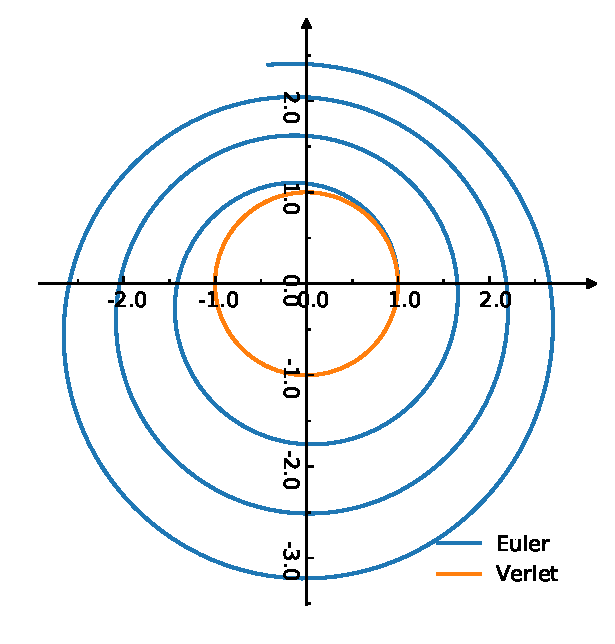
\includegraphics[width=0.7\textwidth]{Earth1000.eps}		\caption{$h = 0.01$year}
		\label{fig:earth1000}
	\end{subfigure}
~
	\begin{subfigure}[tb]{0.5\textwidth}
		\centering
		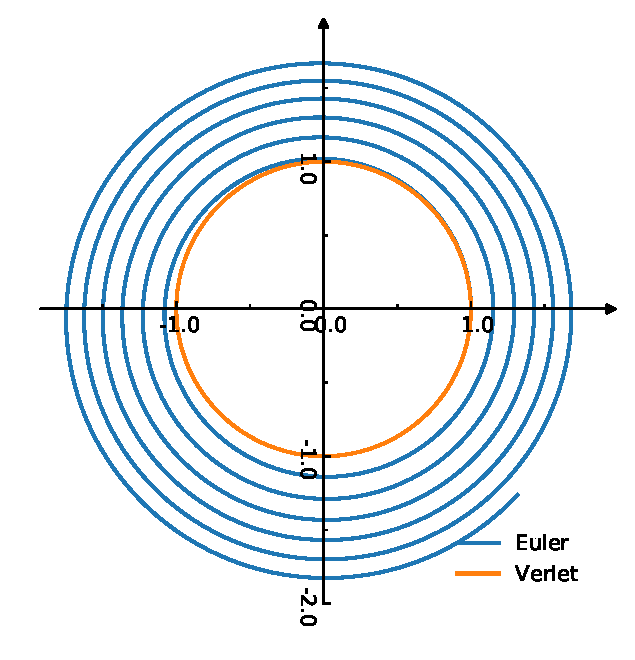
\includegraphics[width=0.7\textwidth]{Earth5000.eps}		\caption{$h = 0.002$year}
		\label{fig:earth5000}
	\end{subfigure}
~
	\begin{subfigure}[tb]{0.5\textwidth}
		\centering
		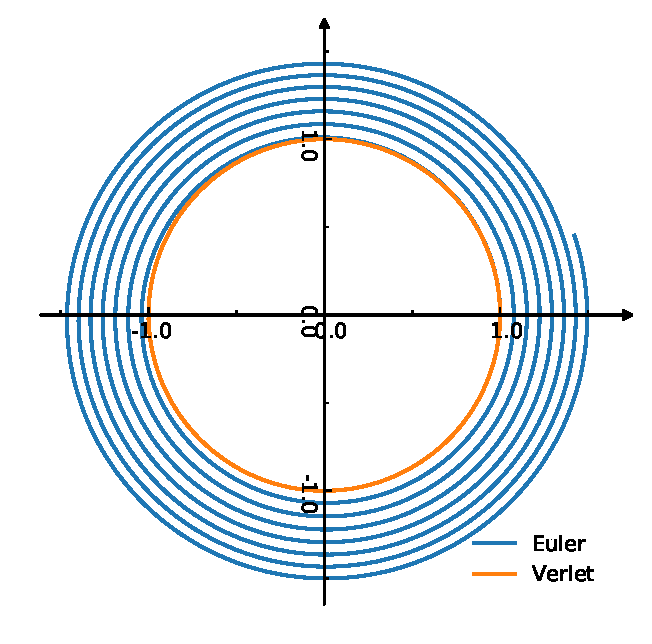
\includegraphics[width=0.7\textwidth]{Earth10000.eps}		\caption{$h = 0.001$year}
		\label{fig:earth10000}
	\end{subfigure}
	\caption{Comparison of different step size $h$ of two methods for 10 years. }
	\label{fig::earth}
\end{figure}

 For detailed check and performance comparison, we list distances, energies, angular momentums together with execution times for these two methods in Table \ref{tab::euler}\&\ref{tab::verlet} with precision up to $10^{-6}$.
 As conservation laws predicted by classical mechanics, physical quantities including kinetic, potential, total energies and angular momentum should be conserved in the Earth-Sun system. 
 From these two tables, we can see conservations in the VV method but not in the Euler method. Thus, we can conclude that the VV method is stable and the Euler method is not.
 
 Compared the execution time of two methods, we find the Euler method is faster. 
 Counting the FLOPS from these two algorithms, we find there is  about 30$N$ for the Euler method and 45$N$ for the VV method. It explains speed advantage of the Euler method.
 
\begin{table}[tb]
	\centering
	\caption{The Euler forward method: step size; kinetic energy; potential energy; total energy; angular momentum in z direction, distance from the Sum and execution time from left to the right.}
	\label{tab::euler}
	\begin{tabular}{ccccccc}
	\hline
	\hline
$h$          & $E_{kin}$        & $E_{pot}$         & $E_{tot}$          & $L_z$        & $r$         & execution time (ms)         \\
	\hline
2.000E-02 & 3.300E-05 & -4.700E-05 & -1.400E-05 & 3.500E-05 & 2.520E+00 & 2.500E-02 \\
1.000E-02 & 2.900E-05 & -4.900E-05 & -2.000E-05 & 3.200E-05 & 2.432E+00 & 5.000E-02 \\
2.000E-03 & 3.200E-05 & -6.500E-05 & -3.300E-05 & 2.500E-05 & 1.824E+00 & 9.400E-02 \\
1.000E-03 & 4.000E-05 & -7.900E-05 & -4.000E-05 & 2.300E-05 & 1.493E+00 & 1.680E-01\\
	\hline
	\hline
\end{tabular}
\end{table}

\begin{table}[tb]
	\centering
	\caption{The Velocity-Verlet method: step size; kinetic energy; potential energy; total energy; angular momentum in z direction, distance from the Sum and execution time from left to the right.}
	\label{tab::verlet}
	\begin{tabular}{ccccccc}
	\hline
	\hline
$h$          & $E_{kin}$        & $E_{pot}$         & $E_{tot}$          & $L_z$        & $r$         & execution time (ms)         \\
	\hline
2.000E-02 & 5.900E-05 & -1.180E-04 & -1.180E-04 & 1.900E-05 & 1.000014 & 2.600E-02 \\
1.000E-02 & 5.900E-05 & -1.180E-04 & -1.180E-04 & 1.900E-05 & 1.000E+00 & 5.600E-02 \\
2.000E-03 & 5.900E-05 & -1.180E-04 & -1.180E-04 & 1.900E-05 & 1.000E+00 & 1.840E-01 \\
1.000E-03 & 5.900E-05 & -1.180E-04 & -1.180E-04 & 1.900E-05 & 1.000E+00 & 3.350E-01\\
	\hline
	\hline
\end{tabular}
\end{table}

For physically meaningful, we will keep using the VV method in our further calculations.

	\subsection{Escape velocity from the Sun}
	In physics, the escape velocity from the Sun is defined as the minimum speed needed for an object to escape from its gravitational influence.
An object starts from the Earth with a initial speed $v_i$. 
Suppose it can goes to infinity far at which potential energy is zero. 
At the same time, it has a minimum kinetic energy zero.
Due to the energy conservation, we can generalize the formula for the escape velocity
\begin{equation}
	\label{escape}
	\frac{mv_e^2}{2} - GM_{\mathrm{S}}m/r = 0\Longrightarrow v_e = \sqrt{\frac{2GM_{\mathrm{S}}}{r}}.
\end{equation}
We can see from Eq. \ref{escape} that the escape velocity $v_e$ is independent of the mass of object.
In our unit system $v_e = 2\sqrt{2}\pi$ which larger than the speed of circular $v_c$ a factor of $\sqrt{2}$.

We would like to use a trial and error method to find the escape velocity.
In our calculation, we fix the step size $h=0.001$ and set up a criteria for escape.
It is if an object doesn't start to turn back after time $t_c$, then it be regarded as a successful escape.
We initialize our calculation the same as in Algorithm \ref{alg::verlet} except a different $v_{y}^0=2\pi \alpha$, where $\alpha$ is a constant larger than 1.
With $1.3<\sqrt{2}<1.5$, we have a lower and upper bounds for $\alpha$ where we can start a binary search for $v_e$.

The results for different $t_c$ are presented in Table \ref{tab::escape}. 
From the table, we find $\alpha/\sqrt{2}$ converges to one as increasing $t_c$. 
Moreover, the total energy gets closer to zero at the same time.
In sum, We would expect $v_e$ and $E_tot$ converge their theoretical value $2\sqrt{2}\pi$ and zero eventually. 

\begin{table}[tb]
	\centering
	\caption{The escape velocity factor $\alpha/\sqrt{2}$ in $v_e=2\pi \alpha$ and total energy for different $t_c$.}
	\label{my-label}
	\label{tab::escape}
	\begin{tabular}{ccc}
	\hline
	\hline
	$t_c$  & $\alpha/\sqrt{2}$          & $E_{tot}$          \\
	\hline
	500   & 0.998968061 & -5.9E-07 \\
	1000  & 0.998418985 & -3.7E-07 \\
	2000  & 0.999002447 & -2.4E-07 \\
	5000  & 0.999456311 & -1.3E-07 \\
	10000 & 0.999655708 & -0.8E-07 \\
	20000 & 0.999781297 & -0.5E-07 \\
	50000 & 0.999879019 & -0.3E-07\\
	\hline
	\hline
	\end{tabular}
\end{table}
	

	
	\subsection{Extension to whole solar system}
	After testing our VV solver for the two-body case, 
we extend our program to solve the Earth-Sun-Jupiter (three-body) system and then the whole solar system. 
This extension is done easily thanks to object-oriented programming. 
Fig. \ref{fig:threebody} shows the orbits of the Earth-Sun-Jupiter system with different Jupiter mass. 
The total time is 100 years. 
In Fig. \ref{fig:leftthree}, when we fix the position of the Sun and set Jupiter mass as $1\times$ and $10\times$ the actual Jupiter mass, 
the orbit of the Earth is still a quite good circle, and we can hardly see any difference between $1\times$ and $10\times$ cases. 
When we do not fix the position of the Sun and fix the center of mass at origin, 
the orbit of the Earth hardly changes. 
So in the above three cases the influence of Jupiter on Earth can be treated perturbatively. 
But when we increase the mass of Jupiter to $1000\times$ (Fig. \ref{fig:rightthree}), 
the Earth flies away and the system seems to be unstable. 
In this case the Sun and Jupiter have almost the same mass, 
and thus the Sun should not be fixed and the whole system is an unstable "binary stars + one planet" system. 
\begin{figure}[tb]
	\begin{subfigure}[tb]{0.5\textwidth}
		\centering
		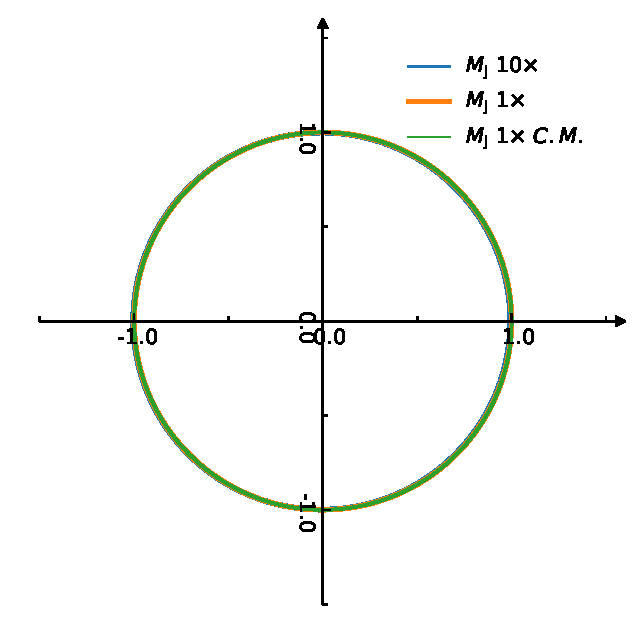
\includegraphics[width=0.7\textwidth]{SEJ_CM.eps}
		\caption{}
		\label{fig:leftthree}
	\end{subfigure}
	~
	\begin{subfigure}[tb]{0.5\textwidth}
		\centering
		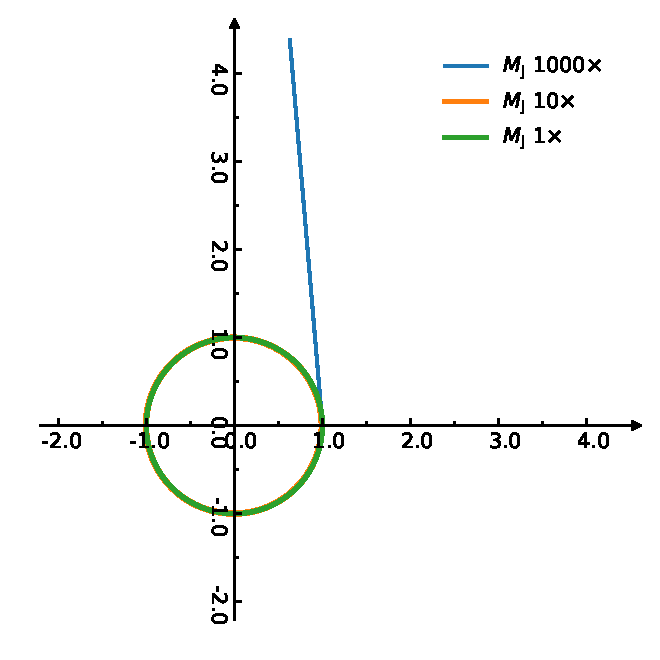
\includegraphics[width=0.7\textwidth]{SEJ.eps}
		\caption{}
		\label{fig:rightthree}
	\end{subfigure}
	\caption{Orbit of the Earth in the Earth-Sun-Jupiter system with different Jupiter mass. 
	C.M. represents that the Sun is not fixed and the center of mass is at origin. 
	Total time is 100 years. The unit of coordinate is AU. }
	\label{fig:threebody}
\end{figure}
\par
After confirming the stability of VV method in the three-body system, 
we simulate the whole solar system using the positions and velocities of the Sun and eight planets 
at A.D. 2018-Apr-02 00:00:00.0000 TDB \cite{NASAdata} as the initial condition. 
Fig. \ref{fig:solarsystem} shows the orbits of the Sun and all the planets. 
The total time is 200 years, longer than the period of Neptune. 
Also, the center of mass is fixed at origin. 
In our simulation, motions in $x$, $y$ and $z$ directions are all calculated. 
But as the motion in $z$ direction is not significant compared to that in $x-y$ plane, 
we only plot the projection of orbits in $x-y$ plane. 
From Fig. \ref{fig:solarsystem}, we can see that the whole system is stable. 
Because of the large mass of the Sun, its orbit can hardly be seen in the figure. 
The orbit of Mercury is not a closed oval because of the impact from otter planets. 
The orbits of other planets are almost closed, and their relative eccentricities agree with the observation. 
\begin{figure}[bt]
	\begin{subfigure}[tb]{0.5\textwidth}
		\centering
		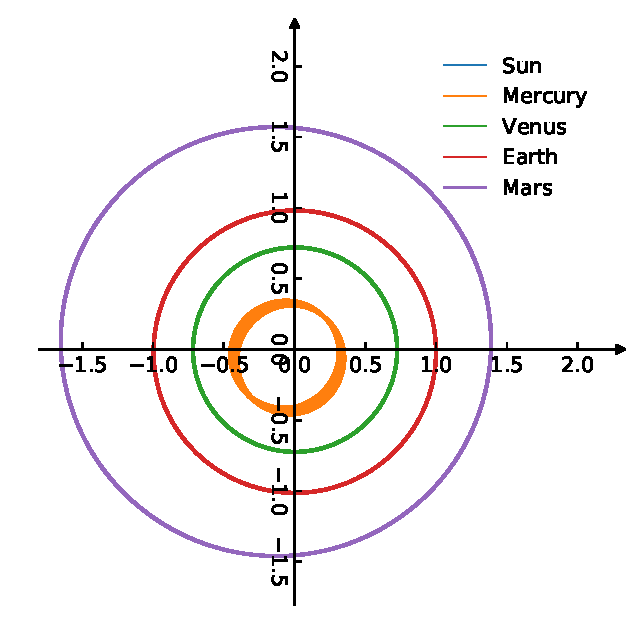
\includegraphics[width=0.7\textwidth]{solar1.eps}
		\caption{The Sun and inner planets. }
		\label{fig:solarinner}
	\end{subfigure}
	~
	\begin{subfigure}[tb]{0.5\textwidth}
		\centering
		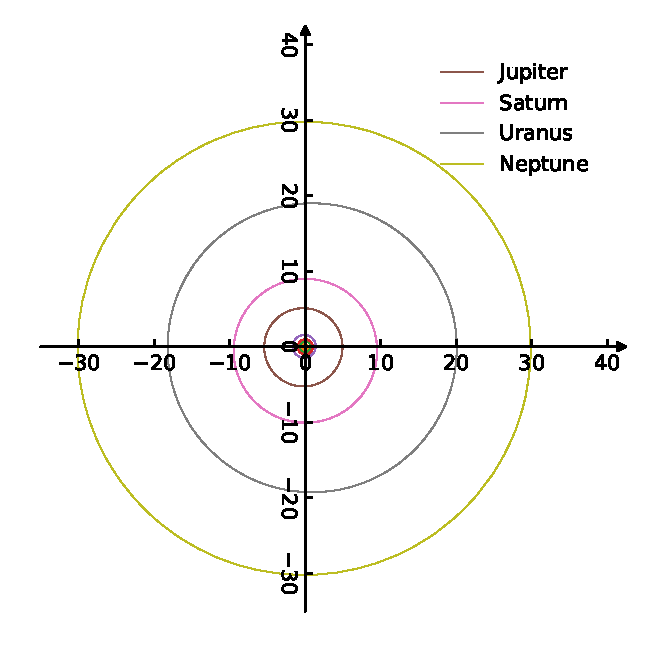
\includegraphics[width=0.7\textwidth]{solar2.eps}
		\caption{Outer planets. }
		\label{fig:solarouter}
	\end{subfigure}
	\caption{Orbits of the Sun and all the planets. The center of mass is fixed at origin. 
		Total time is 200 years. The unit of coordinates is AU. }
	\label{fig:solarsystem}
\end{figure}
	
	\subsection{The perihelion precession of Mercury}
	Historically, the discrepancy between the observed and calculated values of perihelion precession of Mercury were not able to be accounted by classical Newtonian mechanics.
Until the introduction of general relativity, the problem was solved.
It was also labeled as a great success of general relativity.
The value results from relativistic correction is about $\delta \varphi\approx 43^{''}$ per century\cite{wiki:xxx}.
In order to get this value, we introduce a correction to our gravitational force, so that the force becomes
\begin{equation}
	\vec{F}_G = \frac{GM_{\mathrm{S}}M_{\mathrm{M}}\hat{r}}{r^2}\left[1+\frac{3l^2}{r^2c^2}\right],
\end{equation}
where $M_{\mathrm{M}}$ is the mass of Mercury, $l$ is $\vec{r}\times \vec{v}$ and $c$ is the speed of light in vacuum.

In our calculation, we apply the Mercury mass and new force to calculate the acceleration.
The Sun-Mercury system initials from $x_0=0.3075$, $y_0=0$, $v_{x}^0=0$ and $v_{y}^0=12.44$. 
For this elliptical orbit, theoretical calculation gives a period $T_m\approx 0.24073$ yr.
We also notice for a resolution higher to $1^{''}$, we have to use a very small step size.

Before setting up the step size, we did a rough estimation.
The Mercury moves about 420 circles in a century which is about 5.5E08 degrees. 
To distinguish $1^{''}$ within a century movement, we need at least a step size $h$ = 100/5.5E08 $\approx$ 1.84E-07. 
Therefore, $h$ = 1.0E-07 would be a good choice.

We try different $h$ in our calculations and the final results are given in Table \ref{tab::mercury}.
The outcomes justify our estimation that the error will less than $1^{''}$ for $h$ = 1.0E-07.
Eventually, our calculation gives $\delta \varphi=42.9333^{''}$ with $h$ smaller to 5.0E-08 which is very close to the theoretical value 43$^{''}$.
\begin{table}[tb]
	\centering
	\caption{The perihelion precession angle $\delta \varphi$ of Mercury due to relativistic correction after one century. }
	\label{my-label}
	\label{tab::mercury}
	\begin{tabular}{cc}
	\hline
	\hline
	$h$        & $\delta \varphi$     \\
	\hline
	5.00E-07 & 53.2277$^{''}$ \\
	2.00E-07 & 45.8665$^{''}$ \\
	1.00E-07 & 42.8183$^{''}$ \\
	5.00E-08 & 42.9333$^{''}$\\
	\hline
	\hline
	\end{tabular}
\end{table}
	
\section{Conclusions}\label{conclude}
In this work, we investigate two methods, Euler's forward and Velocity-Verlet method, 
to solve a set of first-order ordinary differential equations with initial conditions. 
To test the performance of these algorithms, 
we use them to calculate the evolution of the Earth-Sun, Earth-Sun-Jupiter and whole solar system. 
Our comparison shows that the Verlet method can better describe the characteristics of motion in these systems than Euler's method. 
We conclude that Verlet method is more stable and thus better to use. 
We also use Verlet method to calculate the perihelion precession of Mercury by adding a relativistic correction to the gravitational force 
and obtain a $43''$ per century precession which is the same as the analytical solution. 
	
	\section*{Acknowledgments}
	We are grateful for the sincere guidance from Prof. Morten Hjorth-Jensen. 
	
	\nocite{*} 
	\bibliographystyle{unsrt}
	\bibliography{proj3_ref}
\end{document}